\subsection{Glyph: \glyph{Trigger}}
\label{sec:af:trigger}

A \emph{trigger} is a stimulation that is necessary for the target activity to take place. 

\begin{glyphDescription}

\glyphSboTerm SBO:

 \glyphOrigin Any \glyph{Activity node} (\sect{af:ANs}) or any \glyph{logical operator} (\sect{af:logic}).
 \glyphTarget Any \glyph{Activity node} (\sect{af:ANs}).
 \glyphEndPoint The target extremity of a \glyph{trigger} carries a vertical bar followed by an open arrow pointing to the target activity node (\fig{af:trigger}).


\end{glyphDescription}

\begin{figure}[H]
  \centering
  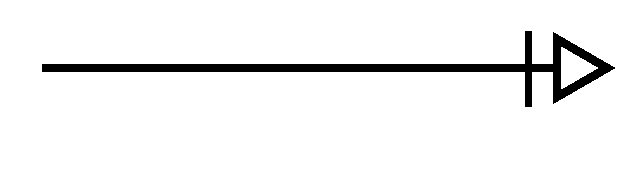
\includegraphics[width = 2in]{images/trigger}
  \caption{The \AF glyph for \glyph{trigger}.}
  \label{fig:af:trigger}
\end{figure}